\documentclass[12pt,a4paper]{article}
\usepackage[a4paper]{geometry}
\usepackage{array}
\usepackage{hhline}
\usepackage{csvsimple}
\usepackage[russian,english]{babel}
\usepackage[utf8]{inputenc}
\usepackage[T2A]{fontenc} 
\usepackage{ulem}
\usepackage{cmap}
\usepackage{makecell}
\usepackage{ifpdf}
\usepackage{graphicx}
\usepackage{wrapfig}
\usepackage[hidelinks]{hyperref}

\setlength\extrarowheight{2pt}
\setlength{\parindent}{0cm}
%
\newcommand{\phylentry}[6] {\\\hline\makecell{
#1\medskip\\
\hhline{|-|}
\\#2\\#3\medskip\\
\hhline{|-|}\\
{#6}}
&\makecell{#4}&\makecell{#5}}
%Syntax: \phylentry{Who}{When}{Where}{Phylosophy}{NotPhylosophy}{ETC} // currently ETC is not used
\hoffset -1.6cm 
\textwidth  16.5cm 
\textheight 24cm 
%\topmargin -1cm 
\parskip 8pt 
\setlength{\unitlength}{1cm}
\sloppy
\addto\captionsenglish{
\renewcommand{\contentsname}{{\bf CO}ntents}
\renewcommand{\refname}{Bibliography}
\renewcommand{\figurename}{Figure}
\renewcommand{\tablename}{Table}
\renewcommand{\abstractname}{Abstract}
\renewcommand{\partname}{Section}
\renewcommand{\bottomfraction}{0.5}
\renewcommand{\floatpagefraction}{0.4}
\renewcommand{\textfloatsep}{0.5cm}
\renewcommand{\intextsep}{0.6cm}
\renewcommand{\floatsep}{0.3cm}
}

\renewcommand\theadalign{cb}
\renewcommand\theadfont{\bfseries}
\renewcommand\theadgape{\Gape[4pt]}
\renewcommand\cellgape{\Gape[4pt]}
%<pics>
\newcommand{\materialist}[0]{\includegraphics{dummy-achievement.png}}%</pics>



\usepackage{float}
\begin{document}
%..................................................................
\begin{titlepage}
\par 
\vspace*{-2cm}
\begin{center}
{\sf \Large
\vspace*{1.5cm}
{\Huge Семенов, 10-й семестр, 2018 }\\
{Наконец, философия без истории, а не история философии и не философия истории}}\\
\vspace*{2cm}
\scalebox{1.2}{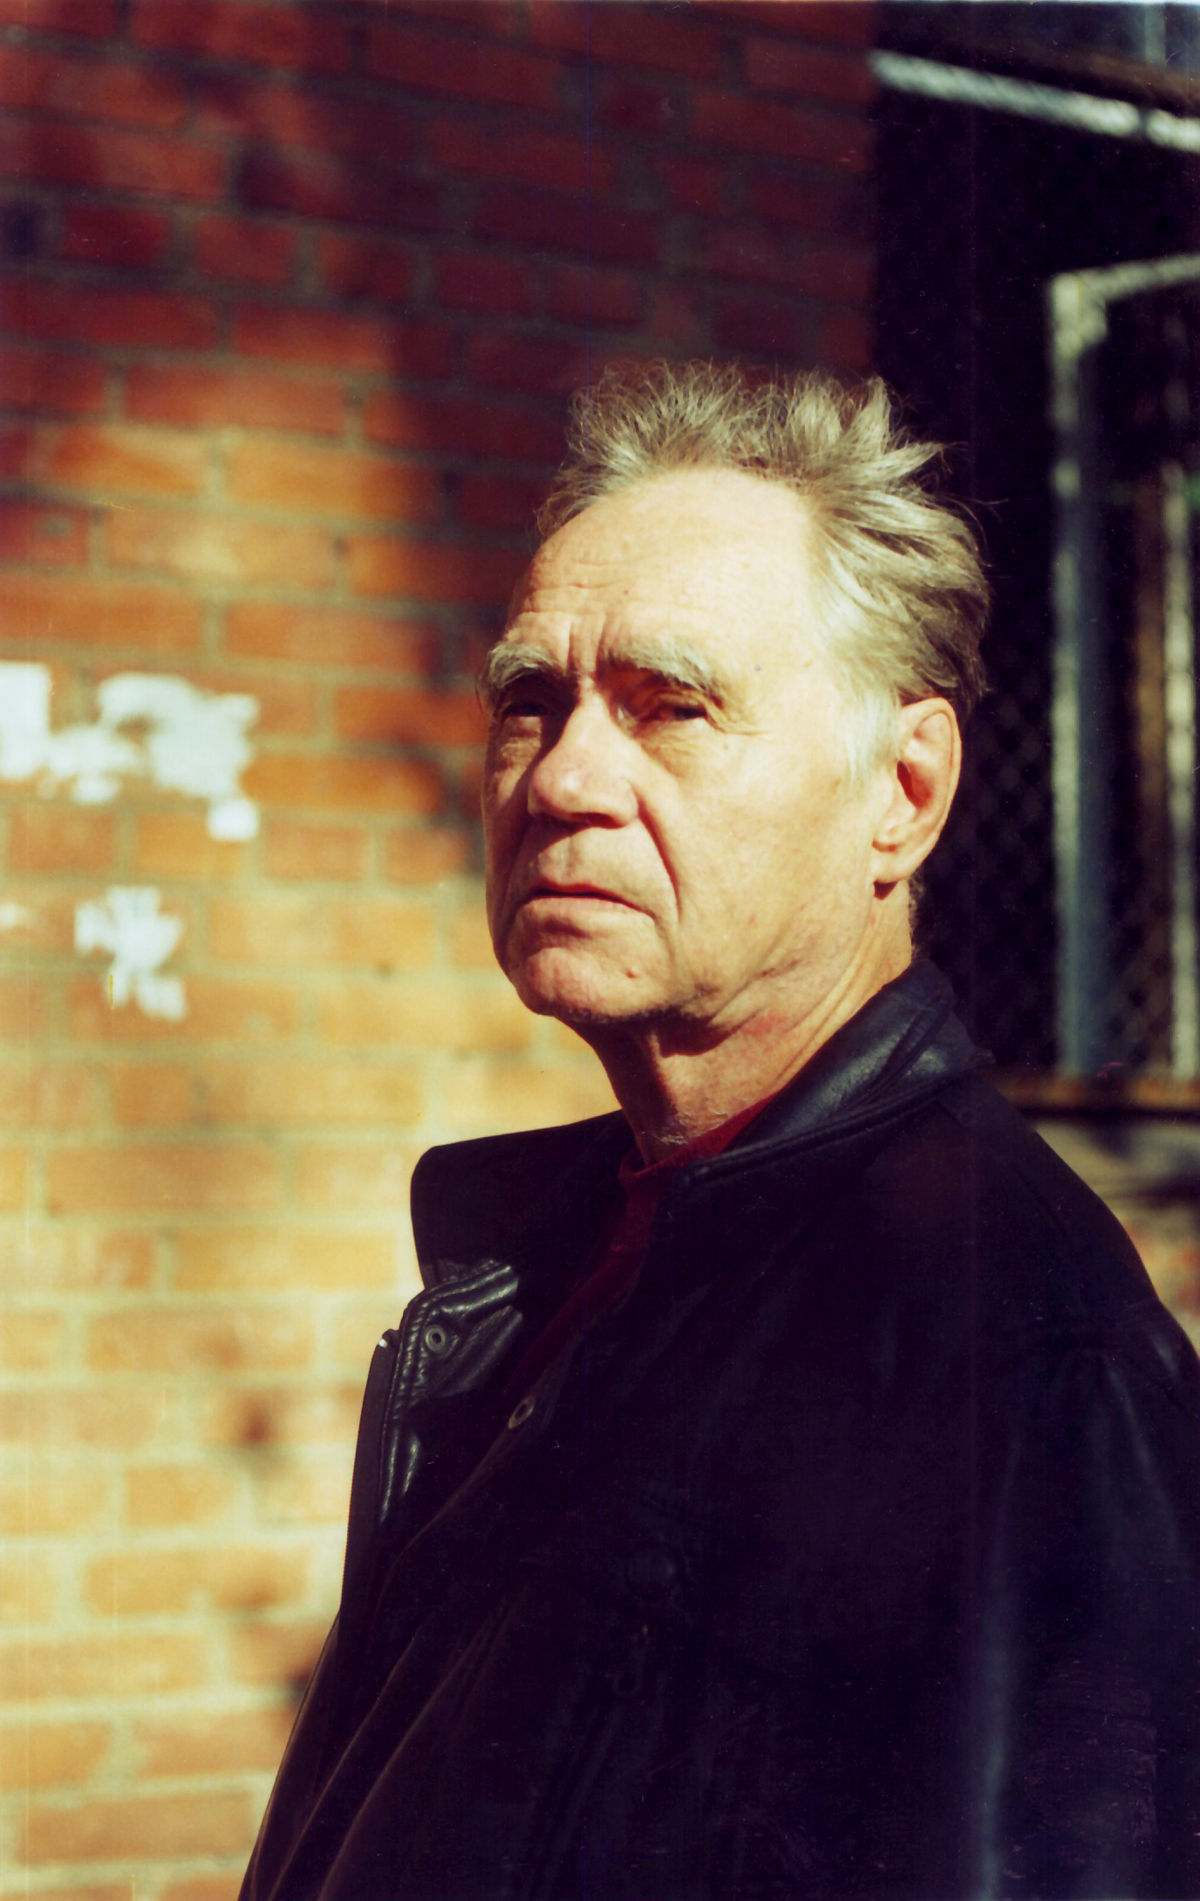
\includegraphics{thegod.png}} 
\begin{flushright}
\sl\small
by Nyaxx11k\\
\end{flushright}
\begin{flushleft}
\hspace{20pt}\raisebox{-33pt}{\scalebox{0.2}{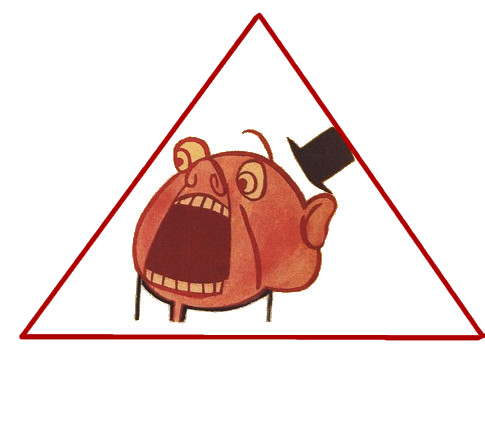
\includegraphics{bourgeois.png}}}
{\itshape Содержит марксизм}
\end{flushleft}
\end{center}
\end{titlepage}
%..................................................................
\topmargin -1cm 
\hoffset -0.7in 
\textwidth 6.0in 
\textheight 9.0in 
\normalsize 
\pagenumbering{arabic}
%----------------
\tableofcontents
%----------------

\section{ Философия как наука об истине, теория познания и самый общий метод исследования.}
Итак, что же такое философия? Если в двух (в четырех) словах, то \textbf{философия} - это наука об истине. \textit{Конечно, любая наука - это об истине (теология - не наука). Но философия - наука об истине в том же смысле, что и биология - наука о живых организмах. Философия ищет истину об истине.} А что мы можем сказать об истине? \textbf{Истина} - это то, что согласуется с действительностью, соответствие между миром и сознанием. Это \textbf{классическое определение истины}. Философия же изучает, как достичь истины, а не заблуждения (\textit{Еще раз, избалованные матлогикой читатели: антипод истины - это \textbf{заблуждение}. \textbf{Ложь} же есть намеренное введение в заблуждение.}). А значит, философия изучает познание, то есть является теорией познания, и она же разрабатывает наиболее общий метод познания, то есть она - наука об этом методе, методология познания. Познание же имеет две ступени - чувственное и мышление. Разрабатывать метод имеет смысл только для второго, ибо первое - это ко врачам. Значит, философия дает наиболее общий метод мышления. Т.е. она еще и наука о наиболее общем методе мышления - \textbf{логика}. Но она же является и самими наиболее общими методами познания и мышления! А еще она онтология. Но это уже третий вопрос. Ибо для него потребуется \textbf{основной вопрос философии}.

\section{ Основной вопрос философии.}
Сразу же ответим: \textbf{"Что первично - мир или сознание?"} Но, спрашивается, почему же он основной? Все дело в том, что мир и сознание надо аккуратно определить - интуитивно-то они и дураку очевидны. Определение дается обычно через род и видовое отличие - "Студент - учащийся (род) высшего учебного заведения (видовое отличие)", "Петух - самец (видовое отличие) курицы домашней (род)". Мир и сознание - два предельно общих понятия, еще более общее - это \textbf{бытие}. Оно включает все. Поэтому содержание утверждения "что-то есть бытие" - это ничто (\textit{Да, про Гегеля правильно вспомнили}). Поэтому так определить мир и сознание нельзя. Можно определить только оба разом, показав отношение между ними. Мир первичен, сознание вторично. Но это у \textbf{материалистов}. Есть еще \textbf{идеалисты}, у которых первично сознание. Причем их три типа - в зависимости от того, б-жественное, мое или общественное сознание в основе всего. Есть еще \textbf{агностики} (хз что первично), \textbf{дуалисты} (оба первичны), \textbf{плюралисты} (много первичного), \textbf{терциалисты} (оба вторичны, а первично что-то третье). \textit{Еще есть те, кто отрицает основной вопрос. Это лжефилософы.} Да, далее нам потребуются термины \textbf{субстанция} и \textbf{акциденция}. Первое - это вещь, которая для существования ни в какой другой вещи не нуждается (\textit{мир/мозг/флешка/кошка (такая-то)}), второе - это то, что существует не само по себе, а в чем-то отличном от него (\textit{сознание как порождение мозга/философия как теория в сознании человека, которое есть продукт мозга/установочный образ линуха на флешке/кошка, но не конкретный Барсик или Мурзик, а кошка вообще}).

\section{ Материализм как онтология и как гносеология. Понятие материи.}
А раз философия отвечает на главвопрос, то она же дает наиболее общую картину бытия, т.е. является \textbf{мировоззрением} ака \textbf{онтологией}. Раньше еще была \textbf{натурфилософия}. Она пыталась дать наиболее общую картину природы, когда все эти физики/химии только зарождались. В чем-то даже угадала (Демокрит с его атомами). Но теперь стала не нужна, \textit{аки тян}. Но осталась еще \textbf{философия истории} ака \textbf{социальная философия}, которая дает наиболее общую картину общества (\textit{ну и пути его развития, разумеется - слово история тут звучит не зря}). А с обществом трудно. Общество - не просто набор людей, а еще и отношения между ними (\textit{точно так же, как и эти ваши интернеты - не только серваки и клиенты, а еще и набор кабелей + набор протоколов TCP, IP, и т.д.}). А есть \textbf{социальные номиналисты} - например, человек и критерий Карл Поппер. Общества нет, есть лишь совокупность индивидов, история - тоже просто совокупность поступков. А противостоят им \textit{социальные реалисты} - они общественные отношения не игнорируют (\textit{Семенов, естественно, здесь}).

Итак, мы подошли к классификации философских теорий. И первый на очереди - \textbf{материализм}. Мир - первичен, сознание - вторично. Для обозначения всего объективно существующего вводится понятие \textbf{материи}. Впрочем, в нашем курсе под материей/материальным понимается только объективная субстанция. Линух на флешке нематериален, но объективно есть. \textit{Кто сказал "Курица - не птица, Убунту - не Линукс?!"}. Для таких ситуаций Семенов использует термин \textbf{объектальное} - объективное, но акциденция, как и идеальное. Так вот, сознание - продукт материального (\textit{мозга, спасибо, \sout{Ева} биология}). Но его вторичность не только в этом. Сознание еще и \textbf{отражает} мир (\textit{не как в зеркале - просто картинкой, а воспроизводит все вещи и объективные законы их движения как может, с погрешностями и ошибками, но все же воспроизводит в отражении.}). Причем не просто отражает, а создает шаг за шагом свой мир ака \textbf{мир-для-нас}. Который, тем не менее, все же копия того, материального мира ака \textbf{мира-в-себе}. \textit{Семенов приводил пример с художником-сознанием, которое рисует картину-для-нас с натуры-в-себе.} Ну и еще сознание
может преобразовывать мир (\textit{но для этого материализм нужно проапгрейдить до диалектического материализма}). Опять же, преобразует оно мир посредством движений материального человеческого тела. Так что тут ни разу не идеализм. И напоследок - философия - это не просто "Что первично, что вторично". Это еще и наиболее общий метод исследования (см. выше), который также напрямую подчинен основному вопросу. Кто движет историю? У идеалиста - великие люди (в такой же идеализм скатывались и французские материалисты). Ну или абсолютная идея. А у материалиста-марксиста - развитие производственных сил и отношений (материальное), порождающее классовые противоречия со всеми вытекающими отсюда революциями (которые хоть и совершаются людьми, но из-за объективных предпосылок). 

\section{ Субъективный идеализм. Солипсизм.}
А теперь пошли по \textbf{идеалистам}. Первый - \textbf{субъективный}. В основе мира - мое сознание (\textit{именно мое, так и говорим на экзамене}). Ну казалось бы, весь мир дан нам только в чувствах и находится в нашем сознании. Значит, быть - значит быть воспринимаемым. Мир находится целиком в моем сознании (\textit{Кто скажет "не существует" - полетит на пересдачу. Мир еще как существует - но в моем сознании}). Казалось бы, что может пойти не так? 

А не так буквально все. Мир в моем сознании. А почему не в твоем? Не в его/ее/\textit{какие там еще местоимения новые левые придумали для списка из 64 гендеров}. У других людей сознание вроде как и у меня. И каждый говорит - "Мир в моем сознании". Но такая асимметрия - это полбеды. Вошел я в комнату. Вышел. Вещи в ней не воспринимаю. Они, стало быть, пропали. Не существуют. Потом я вхожу - оп! - опять существуют. На тех же самых местах, гады, где я их расставил. А уж когда я ложусь спать - так это вообще катастрофа! Впрочем, сейчас мы эту проблему порешаем. Другие люди бодрствуют, вот мир и не схлопывается в небытие. Стоп, а люди не должны тоже исчезнуть? Ведь у них же не мое${}^\mathtt{TM}$ сознание! Это \textbf{солипсизм} - существую только я, а все остальные существуют только в моем сознании. А, неважно. Тут еще одна проблема. Вот я могу съесть яблоко. А могу представить, что съел, и благополучно двинуть концы с голоду. Как определять, воображаемое яблоко я съел, или IRL съел. Стоп, какое IRL, мое сознание и есть IRL! Ну, представление, оно такое блеклое, а IRL оно яркое. Ага, набравшись ЛСД, нарк сигает с крыши, и в его сознании летит вперед. IRL тоже летит, но вниз, и, как правило, долетается до летального исхода. Беркли, запиливший сей сорт идеализма, ввел Б-га, работающего как Абсолютный дух. А это следующий вопрос.

Но перед этим нужно все-таки понять, где в сей концепции рациональное зерно. А оно в том, что мир существует в нашем сознании. Но он существует \textbf{не только} в нашем сознании, он и вне него. От непонимания этого факта и вырастает такой вот идеализм.

\begin{figure}[h]
\scalebox{0.56}{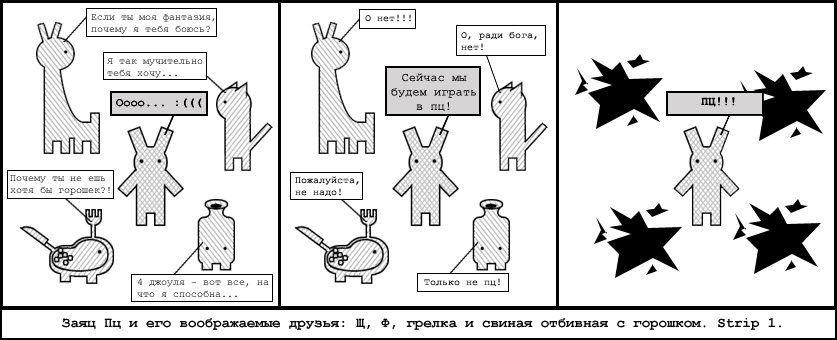
\includegraphics{ptz.jpg}}\\
\caption{Линор Горалик знает толк в солипсизме}
\end{figure}

\section{ Объективный идеализм. Его онтология и гносеология. Основные компоненты.}
Второй идеализм - \textbf{объективный}. В нем есть абсолютный дух - это его сознание порождает мир. Оно уже творит природу, в которой есть другие мыслящие духи - наши сознания. Они уже воспринимают природу, и для них она объективна.

В принципе, это все. Но этого сто процентов мало, поэтому держите историю идеализма. Создателем объективного идеализма был Платон. Он отделил слово от понятия, и встал вопрос - общие понятия существуют, и если да, то где? Ну он и ввел \textbf{идеи} ака \textbf{эйдосы}, образующие целый мир. Причем этот мир первичен, а наш бренный - это его "тень" (притча про пещеру и людей, видевших только тени - это оно). То, что общее действительно объективно, но существует лишь в отдельном, Платон не дошел. Ну и доразвивался так объективный идеализм до Гегеля с его Абсолютной Идеей. Развитие мира - это процесс познания абсолютной идеей самой себя. Окончательно она познала себя в философии Гегеля. Произойти при этом должно было то же, что и когда Беркли лег спать. ИЧСХ, оно же и произошло. Ничего. Объективный идеализм стал противоречить сам себе.

\section{ Агностицизм, или феноменализм.}
Еще одно направление - \textbf{агностицизм} ака \textbf{феноменализм}. Его создатель - Д. Юм. Он говорил, что раз познание вещи - это ее вхождение в сознание, то знаем мы только содержание нашего сознания. А мир - это как раз то, что может войти в сознание целиком. Поэтому что там с миром, мы знать не можем. Есть он только в моем сознании, в сознании Абсолютного д-ха или он вообще объективен - это хз. В сознании он точно есть, а остальное мы не знаем (\textit{Еще раз. Агностицизм - это не когда ничего не знаем. Это когда знаем только содержание своего сознания.}) Итого 3 гипотезы - субъективный идеализм/объективный идеализм/материализм. С точки зрения формальной логики неопровержимо. Но это не значит, что вообще неопровержимо. Чайник Рассела тоже неопровержим, но любому нормальному человеку ясно, что никакого чайника на геостационарной орбите нет. Юма можно опровергнуть созданием теории. Теория всегда основывается на фактах, и часто на их обобщении (см. далее), а уж что-то, а индукция в формальной логике не работает (\textit{пример с белыми лебедями, индукцией и ее опровержением черным лебедем в Австралии}). Так что, если объяснить, что сознание - продукт мозга, построить последовательный материализм, который будет объяснять наблюдаемые явления, и скажет, что отражение мира все-таки находится в сознании, то агностицизм отпадет сам собой. А Семенов на лекциях именно такой материализм и читает. 

\section{ Обыденное и концепциональное знание. Проблема источника концепциального знания. Предлагаемые ее решения.}
Знание бывает разное. Обрабатывал древний человек землю для растений. Не распахал - не взошло. Не полил - не взошло. Топтал - не взошло. Посеял в неправильное время - не взошло. Вот такое бессистемное нагромождение знаний как вести земледелие. Это - \textbf{житейское знание} - бессистемный опыт, получаемый в ходе практической деятельности. Его антипод - системное знание. Научное? Да не совсем, теология тоже в этот антипод попадает. Антипод тут - концепциальное знание - знание, основанное на системе понятий ака \textbf{концепции}. Научное знание же еще и опытное, теоретическое и доказательное. \textit{И работает, в отличие от теологии}.

Источников знания со времен Бэкона (который Роджер) выделялось 3 вида - авторитет, ум и опыт. Реально полагаться можно только на последний. И тут выделились два направления - \textbf{эмпиризм} и \textbf{рационализм}. Первый считает, что единственное знание - это знание, основанное на опыте, т.е. \textbf{апостериорное}. Среди него отдельно выделяется \textbf{сенсуализм} - это направление, утверждающее, что все знание содержится только в чувствах. Нет ничего, чего не было бы в чувствах. А второе направление - рационализм - утверждает, что есть знание, полученное без опыта - \textbf{априорное} - более того, оно является высшей формой знания.

А реальность, как всегда сложнее. Единственный источник информации о мире - это чувства. Сначала идут \textbf{ощущения} от органов чувств - их пять типов (зрение, слух, обоняние, вкус, осязание). Потом они сливаются в единое \textbf{восприятие} вещи. Потом образ этой вещи можно вытащить из памяти - это \textbf{представление}. Но чувства дают материал мышлению, которое уже строит на его базе гипотезы/теории. Так что и тут эмпиристы с рационалистами ухватили по одной стороне истины - одни поняли, что все знание строится на основе опыта, другие - что есть не только \textbf{чувствозримое}, но и \textbf{умозримое} - атомы, например.

\section{ Эмпиризм. Понятия апостериорного и априорного знания.}
См. выше. Тут только перечислим эмпириков. Гоббс, Юм, Беркли. Последние двое - вообще сенсуалисты. Локк еще был, только целиком последователен не был - было у него очевидное знание.

\section{ Ступени человеческого познания.}
Итак, уже было сказано, что познание делится на чувственное познание - о нем уже все сказано - и мышление. Мышление же делится на рассудочное, которое действует по законам формальной логики, и разумное, которое действует по \textbf{содержательной} ака \textbf{философской} логике.

\section{ Чувственное познание и его формы.}
См. выше. Его формы - как раз ощущение, восприятие и представление. Ну и чувственное познание человеку неподвластно. \textit{Нельзя силой воли начать воспринимать ультрафиолет, например. Самый максимум - это отвернуться и начать смотреть на что-то другое. Но это уже не про чувственное познание, а про выбор объекта познания.}

\section{ Сенсуализм и его основные виды.}
См. выше. Итак, знание дано нам только в чувствах. Мышление они не отрицают. Отрицают лишь только, что оно дает новое знание. Сенсуалистами были Беркли, Юм, французские материалисты. \textit{Возможно, Бэкон и Гоббс, хотя и не очень последовательные} Т.е. этого самого сенсуализма 3 вида - субъективный идеалистический/агностический/материалистический, по ответу на главвопрос философии. У первого ощущения - это единственное, что существует, у третьего это лишь результат действия материальных вещей. Второй, как всегда, не знает и никогда не узнает.

\section{ Проблема природы ощущений и восприятий.}
Итак, выше уже были расписаны три вида сенсуализма. Они по-разному объясняют природу ощущений (и восприятий - она точно такая же, поэтому дальше говорим только об ощущениях). Хотя, тут даже четыре точки зрения. Материализм (и наука) говорит, что они - результат действия вещей на органы чувств. Еще есть точка зрения Канта - там тоже ощущение создается вещью. Но у Канта ощущение создается непознаваемой вещью-в-себе, и результат абсолютно, никак не относится к самой вещи-в-себе - она непознаваема. У материалистов же ощущение же сообщает о вещи хоть что-то. Ну и еще есть Беркли с его ощущениями, которые ничем не создаются - мое сознание же - это вещь существует, потому что ощущается. И агностики, для которых эта кухня вообще непознаваемая.

\section{ Решение проблемы природы ощущений и восприятий естествознанием и материалистической философией.}
Итак, материалисты первые на очереди. С ними все просто - ощущения возникают в результате действия вещей на органы чувств. Они несут информацию о предмете, то есть являются в чем-то сходными с ним. Но они не являются самим предметом. Именно это и выражается формулой \textbf{"Вещь и ее восприятие - и одно и то же, и не одно и то же"} в лучших традициях диалектики. На самом деле идеальное имеет два разных смысла. Это не только образы внешнего мира (\textbf{иконоидеальные} - сам по себе образ только похож на предмет), но и содержание этих образов (\textbf{дубльидеальные} - они уже "копии" предмета ). Образы - и субъективны, и объективны. Содержание же всегда объективно, но при том существует в субъективной форме.

\section{ Решение проблемы природы ощущений и восприятий субъективным идеализмом.}
Тут тоже все понятно. Ощущение первично. Что с этим не так - расписано выше. Мир дан нам только через ощущения, но из этого не следует, что вещи и есть ощущения. Но заслуга субъективных идеалистов в том, что они поняли, что мир дан нам только через ощущения. Т.е. это решение кратко выражается формулой \textbf{"Вещь и ее восприятие - совершенно одно и то же"}.

\section{ Кантианское решение проблемы природы ощущений и восприятий.}
Вот тут сложнее. Вроде бы материализм. Ан нет - ощущения никак не похожи на вещь в себе. Мышление, по Канту, пытается упорядочить ощущения, и тем самым творит мир-для-нас. Он на мир-в-себе никак не похож. Тут формула \textbf{"Вещь и ее восприятие - совершенно не одно и то же"}. Тут тоже есть рациональное зерно. Мышление действительно творит мир-для-нас. Но творит его, отражая мир-в-себе.

\section{ Юмистский ответ на вопрос о природе ощущений и восприятий.}
Вот тут самое простое.  \textbf{"Вещь и ее восприятие - одно это и то же, не одно и то же - не знаем, и никогда не узнаем"}. Опять же, для того, чтобы дать ответ на этот вопрос, нужно выйти за рамки восприятий. А мы этого сделать не можем. 

\section{ Как философы открыли, что мир существует в сознании человека? (элеаты, Демокрит, Т. Гоббс, Дж. Локк, Дж. Беркли, Д. Юм, И. Кант).}
Вот тут мы возвращаемся к истории философии. Первыми были элеаты. А именно, Парменид. Решив, что раз бытие - это то, что есть, а небытие - это то, чего нет, Парменид решил, что небытия нет. А значит, бытие неделимо - его части должно отграничивать небытие, да и бесконечно оно, да и неподвижно - части относительно друг друга перемещаться могут. И ничего не появляется/не исчезает - ведь это значит уйти в небытие. Но чувства-то говорят об обратном! Тут Парменид и поделил познание на чувства и мышление. И мышление, понятно, более высокая ступень - чувства какое-то движение суют! Потом его ученик Зенон Элейский своими апориями боролся с движением. Где-то софизмы, где-то единство противоположностей и диалектика. По другому пути пошел Демокрит. У него были атомы, и все свойства вроде цвета/вкуса/запаха он отрицал - говорил, что это просто форма у атомов так ощущается. Есть легенда, что к старости себе глаза выколол, ибо не нужны. Сходные идеи выдвигал материалист Гоббс. А Локк ввел \textbf{первичные} и \textbf{вторичные} качества. Первые объективные, вторые субъективные. Первые есть на самом деле, вторых нет - они чисто порождение сознания. И у всех тут прослеживается идея, что мир в сознании не такой, как на самом деле. Значит, мир есть и в сознании, и мир в сознании не такой, как и мир вне сознания. 

По другому пути пошел Беркли. Он почувствовал, что мир в сознании - это мир вне сознания, и абсолютизировал сходство. У него мир буквально существует исключительно в моем сознании. Что-то похожее у Юма. Но если у Беркли мир точно только в моем сознании и нигде больше, то у Юма он в моем сознании точно есть, а вот есть ли он где-то еще - я знать не могу, потому что он вне моего сознания - в этом плане он преодолевает абсолютизацию Беркли. А уж Кант скатывается в другую крайность: в сознании человека есть мир, но он ни разу и ни в чем не мир-в-себе.

\section{ Что значит знать о чем-то, иметь знание о чем-то?}
Это еще у Юма было. Знать вещь - значит, иметь эту вещь содержанием своего сознания. То есть мир в сознании, мир-для-нас - это все познанное. И возникает вопрос, очень похожий на предыдущий. Мир-в-себе и мир-для-нас - они вообще как соотносятся?

\section{ Наивный реализм.}
Первое решение этой проблемы. Мир вне сознания, и никак не в сознании. Идея, зародившаяся по-видимому еще в ходе практической деятельности первобытных людей по превращению камней в рубила. Действительно, если мир сопротивляется нашим желаниям, если его нужно преобразовывать - камни там раскалывать, то значит, мир находится вне сознания? Рациональное зерно есть, но то, что мир не только вне сознания, поняли еще греки - см. выше.

\section{ Феноменализм. Можно ли его опровергнуть? Можно ли доказать, что мир существует не только в сознании, но и вне него?}
См. вопрос про агностицизм и феноменализм. Его решение проблемы - мира-в-себе и мира-для-нас навеки останется загадкой. Доказательство того, что мир существует вне сознания - это то, что мир приходится преобразовывать - этому нас учит вся практическая деятельность - для достижения желаемого мир нужно преобразовывать, следуя определенным правилам - а не то он преобразуется во что-то другое. Это стало ясно еще с того момента, как первобытным людям потребовалось колоть камни, чтобы у них были острые края. 

\section{ Проблема отношения вещей в себе и вещей для нас. Кантианское и материалистическое ее решение.}
Следующее решение проблемы - кантианское. Собственно, даже вещи-в-себе и вещи-для-нас ака \textbf{ноумены} и \textbf{феномены}- его термины. Кантианское решение проблемы - мир-в-себе и мир-для-нас вообще не пересекаются. Да, воздействуют на нас. Нет, ощущения тем не менее никак не похожи на вещи-в-себе их вызывающие. Поэтому Кант и идеалист - у него мир-для-нас строится мышлением. Тут похожее решение предлагает материализм. Ощущения вызываются вещами. Но главное отличие - ощущение несет о вещи какую-то информацию, а значит и мир-для-нас пересекается с миром-в-себе. Но очевидно, что всегда есть непознанное, а есть наоборот, выдумки. Поэтому ни один из миров не содержится в другом полностью. Ну и ясно, мир-для-нас постоянно расширяется - по мере накопления новых знаний.

\section{ Материализм о вещах в себе и вещах для нас. Познание как превращение вещей в себе в вещи для нас.}
Основное сказано выше. Поэтому сосредоточимся на превращении вещей-в-себе в вещи-для-нас - а именно это и есть процесс познания, ведь знать - значит иметь содержанием своего сознания. Перестает ли вещь-в-себе при познании быть вещью для нас. Угадайте, что про это скажет диалектика? \textbf{И перестает, и не перестает}. И как всегда, необходимо раскрыть, где перестает, где не перестает. Слово вещь-в-себе имеет два смысла. Первый - вещь, которая находится только вне сознания. Второе - вещь, которая просто находится вне сознания. \textit{Это не просто два разных определения - они взаимопроникающие. Действительно, полностью вещь-в-себе никогда не войдет в сознание. Пример - электрон от Ильича. Сложный, бесконечно делимый и неисчерпаемый. ИМХО имеется в виду электрон как предмет познания, но пруфов не будет. Но худо-бедно она может отражаться в сознании - а отражение в чем-то сама вещь, а в чем-то нет. Вещь-в-себе и вещь-для-нас - чистые абстракции, а ИРЛ в каждой вещи в какой-то степени есть признаки обеих (ну если только вещь хоть как-то познана).} Как вещь сугубо вне сознания - перестала. Как вещь просто вне сознания - не перестала.

\section{ Соотношение мира для нас и мира в себе.}
См. выше. Соотношения вещей и миров в-себе и для-нас приходится выяснять параллельно.

\section{ «Теория символов» Г. Гельмгольца.}
\underline{Йоханнес Мюллер (1801-1858)} исследовал органы чувств. Как зрительный нерв не раздражай - будет свет и т.д. 
Г. Гельмгольц и сказал, что ощущения есть, но на предметы совсем не похожи. Это - только знаки, символы, и информации о мире они не несут. Но тем не менее, мышление у него может дать знание о мире. Значит, полностью в кантианство он не ударился. Дюбуа-Реймон говорил, что знание принципиально ограничено. Что-то мы знаем, а что-то не узнаем никогда. Даже книгу "Семь мировых загадок" написал. Символы - материальны, но это только знаки. Тут идея вообще похожа на Демокрита/Гоббса/Локка - нет не цветов, ни запахов - просто чувства приукрашивают мир.

О знаках даже наука есть. \textbf{Семиотика} или \textbf{семиология}. \textbf{Знак} - это физический объект/явление - чувствозримое, представляющее другой предмет. Знаки бывают:
\begin{enumerate}
\item \textbf{Языковые}. \textbf{Язык} есть любая система знаков.
\item \textbf{Неязыковые}. Они одиночные, и подразделяются еще на несколько типов: \textbf{иконические знаки} - знаки-копии, похожие на обозначаемый предмет (фотография человека как его обозначение), \textbf{знаки-индексы} - "признаки" предмета (дым как символ костра - они связаны причинно-следственной связью) и, наконец, \textbf{конвенциональные знаки} - они просто используются по соглашению (\textit{надкусанное яблоко как символ одной очень известной корпорации - кажется оно самое}). Среди них есть  \textbf{знаки-символы} - они воплощают идею (серп и молот - союз рабочих и крестьян). 
\end{enumerate} 

Только и к ощущениям-восприятиям это неприменимо - они идеальны, а знаки материальные. А у Гельмгольца знаки - это чисто ощущения/восприятия.

\section{ «Иероглифический» материализм.}
Из материализма Гельмгольца вырос особый сорт материализма. - \textbf{иероглифический}. По сути, то же самое, просто символы Гельмгольца переименовали в иероглифы. \textit{В него скатывались многие марксисты - Плеханов, например. Ленин их критиковал, Сталин их расс.. Гм... Ну понятно. И да, Семенов очень сильно против сталинизма, но поддерживает Ленина. Кто там говорил, что Сталин-продолжатель дела Ленина?}

\section{ Знаки и знаковые системы.}
См. выше.

\section{ Два аспекта природы идеального: гносеологический и онтологический. Психофизиологическая проблема.}
У идеального есть два аспекта. Во-первых, сознание возникает как результат работы мозга. Как идеальное соотносится с мозгом, каким материальным процессам отвечает движение мысли? Это \textbf{онтологический аспект}. А другой аспект - это \textbf{гносеологический аспект} - как соотносятся вещь-в-себе и вещью для нас. Он про отношение идеального ко внешнему миру. \textit{Т.е. онтологический - это скорее про то, какие сигналы в мозгу кодируют такие-то мысли, а гносеологический - про то, как соотносится яблоко и его восприятие. В первом случае идеальное выступает как материальное, во втором - как нечто, отличное от материального.}. Онтологический аспект ставит \textbf{психофизиологическую проблему} ака \textbf{mind-body problem} ака \textbf{mind-brain problem}. И тут есть список из пяти (шести, если с подпунктами) решений:
\begin{enumerate}
\item Психофизический дуализм - есть самостоятельный дух и самостоятельное тело, и они взаимодействуют; сли даже не взаимодействуют, то это \textbf{параллелизм}.
\item Психофизический монизм - это два проявления одного и того же.
\item Агностицизм. Nuff said.
\item Материализм-1, он же \textbf{научный материализм}. Человек - физико-химическое тело и точка. Нет никакого психического.
\item Материализм-2. Психическое есть, но оно подчинено физическому.
\item Пофигизм. Психическое-физическое. Просто языковая проблема и все.
\end{enumerate}

\section{ Психофизическая проблема в домарксистской философской мысли.}
Еще у греков наблюдалось несколько соображений: кто-то трактовал душу как материальное (Гераклит), кто-то - как идеальное. Там же впервые зародилась гипотеза о том, что орган мышления - мозг. Правда, многие по-прежнему считали им сердце. Так что онтологическая проблема природы идеального только намечалась. В 17 в., с развитием физиологии, она стала психофизиологической. Появились дуализм (Декарт), монизм (Спиноза) и т.д. (см. выше)

\section{ Психофизическая проблема в современной немарксистской философской мысли.}
Тут обычно у психологов психическое сводится к физическому или вообще отрицается (Ламетри и последователи). Проблема так и не решена. 

\section{ Психофизическая проблема в марксистской философской мысли.}
Мысль - не материальна. "Мысль можно свести к химии, но этим не исчерпывается ее сущность" (Энгельс). "Различие материи и духа относительно, не чрезмерно" (Ленин, разбирая Дицгена). Мысль - продукт мозга, это ясно. Но для решения проблемы недостаточно. В СССР же были проблемы. Ильенков абсолютизировал общественное, не различая \textbf{биоидеальное} (оно и у животных есть) и \textbf{социоидеальное} (только у человека). Были еще идеи, что идеальное есть во внешном мире, вне мозга.
А дальше эта проблема будет решаться еще пять вопросов.

\section{ Учение И.П. Павлова о высшей нервной деятельности. В чем прав и в чем не прав И.П. Павлов.}
Павлов открыл \textbf{рефлексы}. Каждый рефлекс - реакция организма на воздействие среды, осуществляемая при помощи нервной системы. Рефлексы бывают условные (вырабатываются и затухают под действием окружающей среды) и безусловные (врожденные). У высших животных безусловные рефлексы - не само поведение, а его фундамент. Павлов же, как всегда, абсолютизировал свое открытие, и всю деятельность человека свел к рефлексам. У него же есть понятие сигнальных систем. Первая - это формы чувственного познания, вторая - слова (существует только у человека). Обе управляются мозгом. Ошибся он в том, что не понял качественного отличия животного от человека. Человек - социальное существо, и социальное заключено в его духе. Социоидеальное же не сводится к биологическим процесса. \textit{И кстати, рассматривая всю деятельность человека как рефлекторную, Павлов , по сути, отвергал свободу воли}. 
% Спросить про философов-немарксистов

\section{ Два вида идеального: биоидеальное и социоидеальное.}
Про них уже было сказано ранее. \textbf{Биоидеальное} - то, что присуще и животным, и человеку - чувственное познание. У человека есть еще и \textbf{социоидеальное}, например мышление. Оно не сводится чисто к биологии (\textit{иначе детей Маугли бы не было - гены-то человеческие}), хотя не может существовать без мозга.

\section{ Основные понятия теории информации. Природа информации.}
Понятия: \textbf{объект информация} - объект - источник информации, \textbf{получатель информации} - тот, для кого предназначена информация.Для информации необходим материальный носитель - физическое тело (\textit{диск}) или физический процесс (\textit{радиоволны}). У них должно быть несколько состояний/элементов - ни и представляют собой \textbf{шифр/код}.

Сначала, информация \textbf{кодируется} на носитель. \textit{Не возникает и кодируется, а появляется при кодировании - до кодирования есть только объект информации, но не информация о нем}. Дальше возможна перекодировка \textit{(например, из электромагнитных волн в магнитную ленту при записи радиостанции)}. Если же информация достигла получателя и преобразована в доступную для него форму, то это преобразование - \textbf{декодирование}. Носители информации сменяются один другим, а сама информация остается - наборы состояний изоморфны, сохраняется порядок.

\section{ Два вида объективного существования: самобытие и въинобытие.}
Самобытие - объективное существование вещи, для которого она не нуждается в другой вещи. Въинобытие - объективное существование вещи, но в чем-то отличном от нее.
Информация объективна, но не материальна. Она \textbf{объектальна}, или же является \textbf{въинобытием}, а не \textbf{самобытием}: ей необходим материальный носитель, но она к нему не сводится. Общее - тоже \textbf{объектальное}: кошка вообще существует, но только как каждая конкретная кошка.

\section{ Чувственное познание в свете теории информации.}
Теперь можно переходить к чувственному познанию. Когда нервный процесс, несущий информацию от органов чувств, достигает мозга, то происходит его декодирование. Процесс уже существует не только в организме, но и для организма. Организм становится не только носителем, но и получателем информации. Нервный процесс тоже обретает двоякую природу - как материальный процесс в организме, и как процесс для организма, для которого важна только переносимая информация - сам по себе нервный процесс не существует для организма. Информация же для него существует не как информация о внешнем объекте, а как сам внешний объект. Объект для нас \textbf{дубльидеален} - объектальный, существующий для нас как материальный; это идеальный дубль материального. Набор этих ощущений образует \textbf{сенсорный мир}.
%иконоидеальное и дубльидеальное

\section{ Идеальное в чувственном познании.}
Таким образом, образ объекта в сознании зависит не только от объекта, но и от строения и состояния нервного аппарата. Внешний объект же для организма выступает только как самобытие - несущего его нервного процесса для организма нет. Таким образом, нервный процесс выступает еще и как единство объективного содержания и субъективной формы, т.е. является иконидеальным. Итак, биоидеальное - это проявление свойства материального нервного процесса, несущего информацию о  внешнем объекте, существовать для организма как этот внешний объект, и тем самым не только как материальный процесс, но и как субъективный образ данного мира.

\section{ Проблема пространства и времени. Кантианское и материалистическое ее решения.}
Теперь займемся проблемой пространства и времени. Вещи в нашем субъективном мире упорядочены по длине, ширине и глубине. Упорядочены также и события - по времени. Кант, понявший, что мир феноменов отличается от мира вещей-в-себе, увидел, что мир феноменов упорядочен. И две первичные формы порядка, по Канту, это как раз время и пространство. Но он считал, что эти формы существуют только в мире-для-нас, что не так. Время и пространство есть формы бытия материального мира. Они объективны, но не материальны. Это формы порядка вещей, которые существуют в чем-то, отличном от них самих. \textit{Эйнштейн одобряет}.

\section{ Субстанциальная и реляционная концепции времени и пространства}
Субстанциальная концепция - время и пространство существуют сами по себе (греки, Локк, французские материалисты кроме Дидро). Реляционная концепция - время и пространство существуют только в чем-то отличном от них (Декарт, Спиноза, Лейбниц).

\section{ Понятие метафизики. Эссенциализм.}
Мир не только чувствозрим, но и умозрим. Точка зрения, что мир только чувствозрим - \textbf{феноменализм}. Что есть что-то, что дает только ум без помощи чувств - это \textbf{метафизика}. Хотя метафизика -термин многозначный, им пользоваться не так удобно (например, метафизика как взгляд на мир, противоположный диалектике). Поппер ввел термин \textbf{эссенциализм} как противоположность феноменализму. Хотя, вместе с этим Поппер противопоставлял эссенциализм номинализму.

\section{ Открытие умозрения и умозримого (милетцы, элеаты, Демокрит).}
У милетцев было первовещество (вода/апейрон/воздух). Они пытались объяснить, почему мир вечен, но в нем нет ничего вечного. Так в чем же мир вечен? Вот и понавводили первовеществ. А первовещество-то неосязаемо! \textit{У Фалеса "вода" - это не обычная вода. Скорее, обычная вода - одно из проявлений первоначала (как и все вещи). А уж апейрон и вовсе нечто не имеющее аналогов.} Вот и получается, что до первовещества нужно догадываться.

Элеаты пошли по другому пути. Парменид умом "доказал", что движения нет, несмотря на то, что чувства его подсовывают. А значит, есть чувства, а есть мышление. Демокрит атомы тоже мышлением вывел. Все эти рассуждения показывают, что кроме чувствозрения есть еще и умозрение и умозримое.

\section{ Человек как единство духа и тела. Сократ о соотношении духа (души) и тела.}
Еще Сократ говорил, что человек - единство души и тела. Душу он отделял от инстинктов, говорил, что человек должен подчинить их себе, иначе он сам станет рабом своих страстей. У него еще воля была, он, сам того не понимая, поделил ее на телодвигательную и социорегуляторную, но это см. далее. Потом эту точку зрения отстаивал Декарт (а животных он все-таки сводил к машинам). Наивные материалисты отвергали душу, сводя ее к материальному. Но человек все-таки единство духа (идеальное, про него будет далее) и тела (материальное). 

\section{ Понятие духа. Дух как единство познания и воли.}
Дух таки есть. Но \textbf{дух} - это не только познание. Это еще и \textbf{воля} - целенаправленная деятельность, способность противостоять инстинктам. Вообще, ее можно разделить на \textbf{телодвигательную} - способность управлять своим телом, и \textbf{социорегуляторную} - господство социального над биологическим (\textit{Да, ради спасения своих лечь на амбразуру вопреки инстинкту самосохранения - это оно. Стадные животные вроде тоже могут рисковать собой - например, мать спасает своих детенышей от хищника - но эта деятельность уже рефлекторная.})

\section{ Р. Декарт о соотношении духа (души) и тела. Рефлексы и волевые действия.}
Декарт считал человека единством души и тела, а животных - просто телом, практически автоматами (хотя и весьма сложными). Правда, дух у него - не продукт мозга, а что-то параллельное. Животное действительно живет рефлексами, оно не отделяет себя от своей жизнедеятельности. Но у человека есть и волевые действия, которые к рефлексам не сводятся (\textit{Ну например, человек может планировать свою деятельность в долгосрочной перспективе, и ради далекой цели терпеть лишения. Это уже не свести к рефлексам.})

\section{ Чувственное познание как реакции организма (тела).}
Чувственное познание - реакция организма на воздействие окружающей среды; в ней нет ничего волевого и для него не существует метода. Про него уже все было сказано выше.

\section{ Мышление как волевая деятельность человека.}
А мышление - вторая ступень познания - уже волевая деятельность. Оно присуще уже только человеку (\textit{А тут о-о-очень большой вопрос. Вроде как утверждается, что у животных не только есть мышление, а что оно даже отличается от человеческого только лишь количественно, но не качественно. Хотя, можно ли считать мышлением одну только способность к обобщению, это тоже вопрос - а носит ли обобщение у животных волевой характер, тоже большой вопрос.}). Поэтому для мышления уже можно разрабатывать метод. Мышление может через действия достигать цели - в этом случае оно правильное, и не достигать - тогда оно ошибочное. \textit{Им занималась добрая половина философов. Бэкон с "Новым Органоном", Аристотель со старым, Лейбниц со своими правилами для исследователя и т.д.}

\section{ Проблема правильного и неправильного образов действия.}
Действия тоже могут достигать/не достигать цели. Но не всегда это неправильный образ действий. Часто образ действий в сознании правильный, но воспроизвести его не удается из-за отсутствия навыка.

\section{ Проблема правильного образа (метода) мысли.}
См. выше.

\section{ Философия как метод мышления и наука о мышлении (логика).}
Про философию как метод и методологию мышления уже говорилось. 

\section{ Два вида мышления: рассудочное и разумное. Две науки о мышлении: формальная логика и логика философская содержательная).}
У мышления две ступени - рассудок и разум (разделил Платон). У рассудка формальная логика (она вышла из философии, спасибо Аристотелю, но затем стала самостоятельной наукой), у разума - содержательная (Гегель). Разумное мышление - объективный процесс.

\section{ Формальная логика — наука о мышлении как субъективной деятельности человека.}
Про нее было сказано выше. Рассудок - субъективная деятельность, в отличие от разума, который объективный процесс, принимающий субъективную форму. Его и изучает формальная логика. Она не занимается исследованием истины, а только дает правила, которым должна подчиняться деятельность человека, чтобы результатом было постижение истины.
%Про субъективность

\section{ Основные формы рассудочного мышления.}
Их три:
\begin{enumerate}
\item \textbf{Понятие} -
форма рассудочного мышления, фиксирующая существенные признаки предмета мыслью. Его \textbf{содержание} - набор существенных признаков предмета. А все вещи, обладающие этими признаками - это \textbf{объем} понятия. \textit{Семенов часто просит привести пример понятия. Говорим любое существительное. Да, "существительное" - это тоже понятие}.
\item \textbf{Суждение} - форма рассудочного мышления, фиксирующая наличие/отсутствия признака. \textit{В языка выражается повествовательным предложением: "Свобода - это рабство"/"Война - это мир"/"Незнание  - это сила". Вопросительные и побудительные - "Чисти-чисти-чисти!"/"Как я буду вилкой чистить?!" - суждениями не являются.}
\item \textbf{Умозаключение} - связь суждений, заключающаяся в выведении из одного/нескольких суждений нового, еще не известного. Делается это путем дедукции/индукции. Дедукция - выведение из общих суждений частного. \textit{Люди смертны $\wedge$ Тит - человек $\Rightarrow$ Тит - смертен.}
Индукция - выведение из частных суждений общего. \textit{Золото при нагревании расширяется $\wedge$ Железо при нагревании расширяется $\ldots$ $\Rightarrow$ Все металлы при нагревании расширяются.} Индукция бывает как полной, так и неполной. С неполной можно выстрелить себе в ногу (\textit{Все лебеди считались белыми, пока не открыли Австралию, где есть черные лебеди. Ну или поросенок на ферме однажды решил, что хозяин всегда будет приносить ему хавчик и только хавчик. На этом хавчике он и отъелся до того, что хозяин пришел с ножом. Вот так, переборщив с индукцией, можно отправиться на мясо.}).
\end{enumerate}

\section{ Основные законы формальной логики.}
Три закона формулированы Аристотелем, четвертый добавился позднее, он от Лейбница:
\begin{enumerate}
\item Закон тождества. На протяжении всей цепочки рассуждений понятие не должно подменяться.
\item Закон противоречия. Не противоречь сам себе.
\item Закон исключенного третьего. Из А и не-А истинно или только А, или только не-А (а третьего не дано).
\item Закон достаточного основания. Суждение должно иметь под собой достаточное основание - вдруг оно ложно?
\end{enumerate}

\section{ Что дает и чего не может дать формальная логика?}
Итак, формальная логика дает новые суждения, выводимые из старых. Но она не дает принципиально нового знания. Что-то дает индукция, но она по сути уже выход из области формальной логики. Она из единичных фактов делает общие. А факт - это уже содержание познания, а не его форма.

\section{ Открытие Г. Гегелем мышления как объективного процесса и его законов.}
Гегель догадался, что мир есть совокупность \textbf{спонтанных}, т.е. саморазвивающихся, процессов.
Логические процессы в нашем сознании воспроизводят реальные процессы. Т.е. законы развития логических процессов - это наиболее общие законы развития мира.
Гегель открыл мышление как  объективный процесс. \textit{Объективность процесса видна из того, что множество открытий делалось дважды и независимо - например, матан - Ньютон и Лейбниц}. 

Формальная логика со временем отпочковалась в отдельную науку. Философия же стала наукой о мышлении как объективном процессе. 

\section{ Конкретно-реальные и логические процессы.}
Есть несколько конкретных реальных - например, физических процессов. \textit{Тут вода закипела, там вода закипела}. Они движутся по единым законам, и соответствуют одному логическому процессу, раскрывающему их законы движения. \textit{Из-за нагревания в жидкости пошли пузыри, которые неустойчивы из-за давления пара, равного атмосферному}. Есть еще процессы химические, биологические, экономические, социальные и т.д. У каждого - свой логический процесс, оперирующий общими понятиями. \textit{Не вода в таком-то стакане, а жидкость}. Эти понятия относятся к физике/химии/биологии/экономике/социологии и движутся по законам физике/химии/биологии/экономике/социологии.
 
\section{ Частнологические процессы и вселогический (панлогический) процесс.}
Значит, есть логические процессы. Они воспроизводят все остальные.
Рассмотренные выше процессы - \textbf{частнологические}. Раскрытие же законов движения частнологического процесса - это \textbf{панлогический} процесс. Он-то и развивается по наиболее общим законам развития мира, т.е. по законам диалектики. В нем понятия предельно общие - категории, которые и движутся по диалектике.

\section{ Основные части философии Г. Гегеля. Сущность гегелевской абсолютной идеи.}
Гегель писал "Науку логики", поделенную на три части. "Учение о бытии", "учение о суждении" и "учение о понятии".
Все развитие мира у него - это познание абсолютной идеей самой себя. На самом деле это  - открытие объективность развития мышления, но Гегель этого не понял. Ну и еще у него была "Энциклопедия философских наук", в которой эта система излагалась. Наука логики в переработанном и урезанном варианте вошла в Энциклопедию как первый том. А вообще система в энциклопедии такая:

\begin{enumerate}
\item Первый том. Наука логики.  $\rightarrow$ учение о бытии, учение о суждении и учение о понятии.

\item Второй том. Философия природы. $\rightarrow$ механика, физика (+химия), органика. Каждая опять делится на три.

\item Третий том. Философия духа. $\rightarrow$ субъективный дух, объективный дух, абсолютный дух.
Субъективный дух $\rightarrow$  антропология, феноменология духа (краткое переложение одноименной работы), психология. Объективный дух  $\rightarrow$ право,мораль, нравственность. Нравственность $\rightarrow$ семья, гражданское общество, государство. Государство $\rightarrow$ внутреннее право, внешнее право, всемирная история. Абсолютный дух $\rightarrow$ искусство (образная форма познания), религия (в счет идут только имеющие священное писание) и философия. Тут абсолютный дух наконец полностью осознает себя.
\end{enumerate}

\section{ Понятие диалектики. Основные значения слова.}
Слово "диалектика" встречалось еще в Древне Греции. Но нас интересуют следующие его значения:
\begin{enumerate}
\item Диалектика мира - наиболее общие законы движения мира.
\item Диалектика сознания - наиболее общие законы движения сознания.
\item Диалектика как наука с двумя диалектиками мира и сознания.
\item Диалектика как метод мышления.
\end{enumerate}

\section{ Отличие диалектики Г. Гегеля от диалектики К. Маркса.}
Гегель открыл диалектику сознания и догадался до диалектики мира (хотя и отрицал это). Как идеалист, он выбрал за первичную диалектику сознания. А в марксизме наоборот - первична диалектика мира.

\section{ Философия как наука о мышлении и самый общий метод мышления.}
Философия является наукой о мышлении. Она изучает логические процессы - а воспроизводящий их процесс - панлогический - наиболее общий  - он же и соответствует философии. Значит, философия еще и самый общий метод мышления.

\section{ Мышление и язык. Понятие и слово.}
Определение языка дано выше. \textbf{Слово} - один из знаков языка. Его еще называют \textbf{именем}.  
Мышление всегда языковое - слова нет без обозначаемого им понятия, понятия нет без слова/словосочетания. Но они не одно и то же - слово материально, понятие идеально. \textit{Слово обозначает, понятие отражает, и не наоборот}. Слово от понятия отделил еще Платон.  Слово же выражает общее.

\section{ Понятие знака. Треугольник Фреге: знак, предметное значение знака (денотат), смысловое значение знака (десигнат).}
Готтлоб Фреге ввел понятие \textbf{знака}. У него был треугольник, в вершинах у него знак, предметное значение знака - \textbf{денотат} и его смысловое значение - \textbf{десигнат}. Пример: слово "кит" - каждый кит в мире - понятие "кит".

\section{ Проблема природы понятий.}
Для содержательной логики исходным звеном также является понятие. Поэтому и необходимо изучить проблему природы понятий - а именно, выявить их отношение к объективному миру. А это, однако, проявление основного вопроса философии. 

\section{ Проблема общего и отдельного.}
Общие слова есть. А общие понятия? Тут есть три точки зрения:
\begin{enumerate}
\item Номинализм. У него есть два подтечения - крайний и умеренный.
\item Реализм
\item Диалектическое решение проблемы общего и отдельного
\end{enumerate}

\section{ Номинализм: крайний и умеренный (концептуализм).}
Умеренный номинализм говорит, что общее есть в сознании, но что его нет ИРЛ (Локк). Крайний - что общего вообще нет (Гоббс, Беркли, Юм) - есть только слова. \textit{Стало быть, нет и мышления - оно общее}. Часто сбивались от крайнего к умеренному.

\section{ Открытие Платоном понятий и мышления как объективного явления.}
Понятие выражается словом / словосочетанием, и слову всегда соответствует понятие. Казалось, что это одно и тоже. А Платон отделил слово от понятия - это не одно и то же. Тогда и встал вопрос -  общие слова есть. А общие понятия? Вот Платон и ввел мир эйдосов. Эйдосы объективны и образуют объективный мир. Мыслящие духи в людях, когда видят вещи (основа которых - эйдосы), вспоминают, что в мире эйдосов что-то такое уже видели. Отсюда и общее в бренном мире вещей. Опять же, рациональное зерно тут в том, что общее действительно объективно есть. Но оно и не основа мира отдельного, а диалектическая противоположность отдельного, и уж тем более не существует без отдельного, ну и уж точно, не  как особый мир эйдосов. 

\section{ Реализм. Учение Платона о двух мирах.}
Реализм реализму рознь. У Платона общее образовывало отдельный мир, являющийся основой мира отдельного. Это - мир эйдосов. Дух попадает в него, потом в мир вещей, вспоминает, что он видел в мире эйдосов - оттуда и появляется общее. Это крайний реализм. У других (Аристотель, Шеллинг, Гегель) общее существовало только в отдельном. Это умеренный реализм. Но реализм - про то, что общее все же основа вещей.

\section{ Три решения вопроса об отношении универсалий и вещей.}
\begin{enumerate}
\item Universalia post res - общие понятия после вещей. Под этим понимался номинализм (хотя, для крайних номиналистов общих понятий нет).
\item Universalia ante res - общее до вещей. Платоновский реализм (хотя опять же, платонисты не настаивали на том, что универсалии существуют только до вещей). Общее у них было до вещей, в вещах и в сознании (среди реалистов были схоласты, до вещей у них общее было в божественном разуме).
\item Universalia in rebus - общее в вещах. В смысле - только в вещах, так-то оно и у вторых есть в вещах. Умеренный реализм. У Аристотеля, например, форма - активное начало вещи, которое обязано соединиться с материей. Хотя, форма форм - бог - работает у него как вместилище всех форм. Т.е. Аристотель все-таки сползает к платонизму.
\end{enumerate}
А так - есть номинализм, реализм и объектализм. Про него будет далее.

\section{ Два вида реализма крайний и умеренный.}
См. Реализм.

\section{ Материалистический универсизм, или объектализм.}
Есть еще объектализм. Вот о нем и поговорим - про номинализм с реализмом уже сказано. Общее, конечно, объектально - существует только в отдельном и через отдельное. Но и отдельное обязательно несет общее. Т.о. общее с отдельным - диалектические противоположности. И да, общее общему рознь. Менее общее выступает как особенное для более общего.

\section{ Диалектика общего и отдельного.}
Это про противоположности. см. выше.

\section{ Понятия как образы внешнего мира. Два вида бытия общего: в мире и в мышлении.}
Чувственное познание отражает отдельное. Понятия - образы объективного мира, и тоже имеют в нем \textbf{коррелят}. Но понятия бывают общими - коррелят у них тоже общее. Но общее нужно извлечь из отдельного. Чистого общего в мире нет. Есть набор отдельного, в каждом есть общее. Для того, чтобы дополнить это до чистого общего, нужна фантазия - воображение. А значит, у общего есть два вида бытия  - в реальном мире в отельном и в сознании в чистом виде. В сознании общее существует уже как отдельное и само по себе, а не в отдельном. Понятия субъективны по форме и объективны по содержанию. Но тут субъективность - не просто имя/знак. Объективное общее облекается в субъективную форму чистого общего. 

\section{ Понятия как продукты человеческого творчества. Роль фантазии в познании общего.}
См. выше.

\section{ Соотношение чувствозримого и умозримого миров для нас.}
Умозримый мир строится на чувствозримом. Исходный материал дают только чувства, но кое-что (\textbf{например, атомы}) в состоянии дать только мышление. Ну и для упорядочения чувств нужны понятия.

\section{ Чувствоумозримый мир в себе и для нас. Создание чувствоумозримого мира для нас как воспроизведение объективного мира.}
Чувствозримый и умозримый миры составляют чувствоумозримый мир. Точно так же есть чувствозримые миры в-себе и для-нас. В чувствозримом мире-в-себе - все чувствозримые вещи. Отдельных атомов там нет. Когда мы воспринимаем эти вещи, они входят в чувствозримый мир-для-нас. Таким образом, и тут мир-для-нас - постоянно уточняющееся отражение мира-в-себе. С умозримым сложнее. Умозримый мир-для-нас строится на основе чувствозримого мира-для-нас, но все так же отражает умозримый мир-в-себе.

\section{ Понятие факта.}
\textbf{Факт} - это истина, фиксированная в суждении; момент мира, вырванный и пересаженный в человеческую голову и преобразованный в ней. \textit{А еще он ужасно упрямая вещь. Но это к вопросу о его объективности}. Самого по себе его в объективном мире нет. Есть только его коррелят - \textbf{эквифакт}.

\section{ Методы добывания фактов в естествознании: наблюдение, измерение, эксперимент.}
В естествознании факты добываются через наблюдением (поиск, наблюдение, фиксация результатов без вмешательства), измерение (сравнение с эталоном), эксперимент (уже вмешательство в мир для создания необходимых условий). Есть еще история, в которой нет даже прямого наблюдения, а только работа с источниками.

\section{ Первичная обработка фактов. Единичные и общие факты.}
Исходные факты - единичные. Их необходимо интерпретировать - исключительно из единичных фактов теория не строится (даже в истории есть частнообщие факты). Единичные факты обобщаются до общих фактов.

\section{ Объективность и субъективность фактов.}
Содержание факта только объективно, хотя он и существует в сознании, а не в мире (в мире есть его коррелят). Факт не бывает истинным или ложным - он только объективен. \textit{Бывают, конечно, лжефакты - выдуманные "факты", но они ни разу не являются фактами, а только выдаются за них.} Факт не только лежит в субъективной форме, субъективен так же процесс "вырывания" отдельных моментов из мира - ИРЛ они связаны.

\section{ Проблема понимания и объяснения фактов.}
На одних фактах картину мира не построишь. Поэтому факты нужно интерпретировать; факт нужно понять и объяснить, а не просто знать. А что такое понимание - вопрос интересный. Пытались отделить понимание от познания, подключали \textbf{герменевтику} - науку о толковании литературных текстов. Получилась философская герменевтика. Лучше бы не получалась. Понимание фактов - это не наСПГСить скрытый смысл в тексте. Факты сами по себе разрознены. Для получения же картины мира их нужно склеить.

\section{ Интерпретация (истолкование) фактов как их объединение (унитаризация)}
Унитаризация фактов - факты объединяются в единое целое. И у этого слова два разных смысла.

\section{ Два вида унитаризации фактов: холизация и эссенциализация.}
Унитаризация бывает двух видов. Первый - холизация - единичные факты объединяются, склеиваются идеями  в холию ака идейно-фактуальную картину мира - единую картину. Про идею будет дальше. А второй тип унитаризации - это эссенциализация/теоретизация. Объяснить явление - значит раскрыть законы его движения. Эссенциализация как раз про это. Она уже оперирует общими фактами. Эссенциализация уже рангом повыше холизации.

\section{ Теория и теоротекст. Переход от теории к теоротексту (текстуализация) и от теоротексту к теории (интеллектуализация)}
Из идеи рождается система идей - гипотеза - которая создается на основе общих фактов, но проверяется единичными. Если гипотеза прошла проверку, она становится теорией. Про нее тоже будет. Что важно - идея состоит из понятий, а не из суждений. Теория тоже. А еще теория - форма разумного мышления, и ее не следует путать с теоротекстом. Теоротекст - это раскрытие теории в языке. Знать теоротекст - не знать теорию. Превращение теории в теоротекст - это текстуализация. Обратно - интеллектуализация.

\section{ Идея — ключевое понятие разумного мышления.}
Идея - единица понимания/интерпретации факта. Она способна нести истину/заблуждение. Но напрямую ее истинность установить нельзя - только по полученной идеефактуальной картине мира.

\section{ Проблема и идея. Практическая и познавательная идея.}
Сначала были только практические идеи - как решения практических проблем. Познавательная проблема состоит из двух частей - понимание того, что что-то не понятно, и задача - поиск решения. То же самое и с практической проблемой - постановка проблемы - это тоже важный шаг.

\section{ Рождение идеи. Озарение. Интуиция.}
Идея не выводится из фактов напрямую. Она - продукт интуиции (\textit{форма разумного познания, которую мы не осознаем, а не РЕН-ТВ}). Идея приходит "вдруг", в результате озарения. 

\section{ Проблемно-фактуальная интуиция.}
Логика разумного мышления - не только объективные законы. Есть и субъективное движение мысли - это открыли психологи. Тут говорится про особую интуицию - про проблемно-фактуальную. Она основана на знании фактов и труде. Для того, чтобы родилась идея, нужна абсолютная свобода мысли и одаренность.

\section{ Житейская бессознательная и сознательная холизация. }
Холизация часто бывает бессознательной - всегда приходится скреплять факты идеями. Иногда, часть фактов подгоняется под идею, часть выбрасывается - в результате картина мира получается искаженной (мания преследования и т.п.). Рядом с бессознательной холизацией есть сознательная - например, поиск зверя по следам. Такая житейская холизация была еще в древности.

\section{ Профессионально-специализированная (расследовательская) холизация.}
Есть и люди, профессионально занимающиеся холизацией. Например, следователи или ученые.
В исторической науке холизация тоже нужна. Но часто единственные доступные факты - единичные. Проверять такую картину можно только новыми фактами.

\section{ «Философия науки» неопозитивизма и постпозитивизма }
Зародилось это в Венском кружке. Карнап, Франк и т.д. Признавали только чувствозримое. Все знание - в языковой форме. Высказывания могли быть или на языке наблюдений (протокольные высказывания), или на теоретическом языке (универсальные высказывания). Они %?протокольные
 гносеологически первичны, они передают чувственный опыт, они достоверны и они нейтральны по отношению к знанию. Сущность непознаваема. Уже видно, что теорию подменили теоротекстом. Тут же встала задача отделить научные высказывания от ненаучных - проблема демаркации. Нужна она только для теор. высказываний - протокольные истинны. Сначала предложили верификацию - сведение теоретического высказывания к сумме протокольных и их проверку. Но теория не сводится к таковым. Возникла концепция теории - не знания, а инструмента получения знания (которое и так в чувствах!). И чистый опыт, если он фиксируется в словах, уже не чистый - слова сами возникали на основе опыта. Потом Карл ВПоппер предложил фальсификацию - научное высказывание должно быть потенциально опровергаемо. По сути, это равносильно тому, что теория что-то запрещает, и нужно искать ее опровержения (а нужно в равной степени и подтверждения, и опровержения). Проблема в том, что единичным фактом теорию не всегда опровергнешь - вдруг ошибка эксперимента. И понеслась... Куны, Лакатосы, а под конец - Фейерабенд просто послал истину лесом. Видите ли, один думает так, а этот - эдак, а этому магия нравится, а навязывать истину - это вообще тоталитаризм и против прав человека. \textit{Кстати, если нет ничего истинного, то и концепция Фейерабенда...}

\section{ Факты, эссенциальная идея, гипотеза и теория.}
Теория - система понятий, определяющая сущность явлений, раскрывающая законы. Чистой сущности, как и чистого общего, в мире нет, но она отражает реальную сущность. Гипотеза отличается от теории только тем, что теория подтверждена, а гипотеза еще нет. Для того, чтобы раскрыть сущность, нужна эссенциальная идея. 
 
\section{ Способы проверка гипотезы (теории).}
Гипотезу проверяют фактами. Хотя бы один противоречит - отвергается. Искать нужно как подтверждения, так и опровержения.

\section{ Две компонента теории и два пути развития теоретического знания.}
Доказали гипотезу, появилась теория. Потом появилсь факты, опровергающие теорию. Теория состоит из двух компонент - из ядра (главные идеи, без которых теория не может существовать) + второстепенные идеи - периферия (конкретные применения теории).\textit{Это придумал Лакатос. Еще одна здравая мысль постпозитивизма.} Если факты противоречат периферии - необходимо переработать периферию. Получится та же и не та же теория. Если же противоречат ядру - теория распадается. Но при этом, конечно, нужно проверить факты.

\section{ Проблема «теоретической нагруженности» фактов.}
Якобы не теория строится на фактах, а факты являются результатом теории. Бред. Факт может интерпретироваться с помощью теории, в ее системе понятий (не "стрелка у гальванометра отклонилась", а "электрический ток потек"), но сам факт - объективен.

\section{ Теоретическая триада: теория, мир как он в теории (теорозримый мир) и теоротекст.}
Теория - образ внешнего мира. Она и субъективна (по форме), и объективна (по содержанию). Одной теории могут соответствовать разные теоротексты (квантмех). Но теорозримый мир, как содержание теории, один.
Раньше физической реальностью называли мир, какой он на самом деле. Теперь - как мир в теории.

\section{ Истинное, истинность, истина. Объективность истины.}
Тут три понятия. Про истину см. далее. Истинное - несущее истину. Истинность - свойство нести истину. Истина только объективна. Истинным же может быть, например, суждение, субъективное по форме. Но суждение создается, а его истинность - нет, она сама возникает в процессе создания суждения. Так что истина $\ne$ истинное.

\section{ «Корреспондентская» теория истины. Проблема критерия истины.}
Оно же - классическое определение истины - соответствие между миром и сознанием. Соответствие  - как совпадение, а не как конвенциональное соответствие. Познание же - процесс подгонки мира-для-нас под мир-в-себе. Соответственно, встает вопрос - как отделить истину от заблуждения? Наивысший критерий истинности - практика. Истина приводит к успеху, заблуждение - к неудаче.

\section{ Концепции очевидности. Авторитарная концепция истины.}
Истина - очевидное/Истина - то, что утверждают авторитеты. Первое - очевидно, что Солнце движется по небу. А то, что это от вращения Земли, уже не так очевидно. Второе - авторитеты могут ошибаться. \textit{Марксизм категорически против такого подхода. Что самое ироничное, именно в СССР по факту пользовались авторитарной концепцией истины. Неопровержимый аргумент - цитата из классиков. Маркс кроет Энгельса, Ленин кроет Маркса, Сталин кроет Ленина. Сталин, он такой: ты ему цитату, а он тебе ссылку.}

\section{ Концепция общезначимости. Конвенциализм.}
Истина - то,как думает большинство/результат соглашения ученых. \textit{Опровергается тем, что 95 \% - идиоты, а раньше и в лешего верили. А ученые верили в теплород.}

\section{ Концепции простоты (экономии мышления) и когерентности.}
Следует считать истиной более простую теорию/истина - это то, что непротиворечиво. Теория заговора сюда отлично впишется. Хотя, во второй есть доля правды. Если сам себе противоречишь - это точно не истина. Но вот в обратную сторону это не работает.

\section{ Прагматическая концепция истины.}
Истина - то, что приносит пользу. Опять есть зерно истины - руководствуясь ошибочными утверждениями, можно ошибиться на практике. А можно и угадать. А можно врать и зарабатывать на этом - пользу приносит дезинформация. А за правду можно, наоборот, отправиться за решетку (\textit{тут просто парад отсылок к Сталину и сталинизму}). 

\section{ Современный антиверитизм.}
Неопозитивизм истину еще не отвергал, но уже полз к этому. Поппер объявил, что истину от заблуждения не отличить - к ней можно только приближаться. Дальше постпозитивисты забили на истину болт. А Фейерабенд ее вообще отвергал, называл "чудовищем абстрактным", даже права человека (а именно, право нести дичь под маской свободы мнения) подключал. \textit{Даже предлагал изучать по желанию магию вместо науки в школах. А то дофига поддержки от государства этой науке.}

\section{ Проблема суверенности человеческого познания.}
Может ли человек (человечество) полностью познать весь мир? В основном говорили, что нет. Избалованные физикой частиц скажут - "да" - осталось только впихнуть в лагранжиан гравитацию. А правильный ответ - (\textit{нужно больше диалектики}) и может, и не может. Может - в том смысле, что ничего непознаваемого в мире нет. А вот непознанное будет всегда. (\textit{Любителям теоретико-полевого редукционизма на заметку - кроме лагранжиана есть еще начальные/граничные условия, которые целиком не описать}).

\section{ Абсолютная и относительная истина.}
Вот была у нас теория. Работала. И вдруг ее опровергли, построили новую. Старая - истина или не истина? \textit{Ну, угадайте, что скажет диалектика... Или? И!}. Тут нужна теория абсолютной и относительной истины - как абсолютного и относительного соответствия между миром и сознанием. 

\section{ Конкретность истины.}
Абстрактной истины нет - истина всегда конкретна. В самом деле, то, что было в одних обстоятельствах истинным - становится ложным. Истина не зависит от человека, но зависит от места и времени. \textit{Например, фраза "идет дождь". Или утверждение о том, что дождь полезен для сельского хозяйства}.

\section{ Граничность (предельность) истины.}
Любое истинное мыслетворение истинно только в определенных рамках. Тут уже не только место и время. Тут уже границы применимости - как у классической механики, например. Так истинное утверждение можно до абсурда довести (что и делали Кант, Беркли и т.д.).

\section{ Диалектика истинного и ложного.}
Итак, истинное и ложное неразрывно связаны друг с другом. Они взаимопроникают друг в друга. \textit{Но не истина и заблуждение}. Это показано выше. Познание истины чревато скатыванием в заблуждение. Грань между истинным и ложным относительна, но все же она есть.

\section{ Истинное и ложное в развитии мировой философской мысли. Ложноистинные концепции.}
Тут разве что про идеализм сказать. Он - не глупости и не религия, а раздувание одной из граней истины. Разумеется, каждая отдельная линия развития человеческого знания ведет в итоге к заблуждению. Но в ней может быть и зерно истины. Это ложноистинная концепция.
 \end{document}